\section{РМК}
\subsection{Объекты тестирования, описанные в разделе}

Тестирование рабочего места кассира нужно проводить на кассе и только при подключенном оборудовании ( фискальные регистратор, сканер штрихкодов, весы, табло покупателя)
\begin{longtable}{p{0.05\linewidth}p{0.4\linewidth}p{0.4\linewidth}}
    %  \toprule
    \hline
    1 & Вид объекта & Обработка \\
    \hline
    %     \hline
    %    \endhead
    & Имя & РМКУправляемыйРежим \\
    \hline
    & Синоним  & РМК (управляемый режим) \\
    \hline


    \bottomrule %%% верхняя линейка
\end{longtable}

\newpage
\subsection{РМК (управляемый режим)}
\renewcommand{\arraystretch}{1.8} %% расстояние между строками таблицы
%\begin{landscape}
\begin{longtable}{|p{0.02\linewidth}|p{0.3\linewidth}|p{0.3\linewidth}|p{0.3\linewidth}|}
    %  {|c|c|l|c|}
    \hline
    № & \textbf{Действие} & \textbf{Ожидаемый результат} & \textbf{Фактический результат} \\
    %****************************************************************************************************
    \hline
    \hline
    \endhead
    \multicolumn{4}{|c|}{\textbf{\textit{Проверка запуска РМК при старте}}} \\
    \hline
    \Rownum & Запустить конфигурацию магазина  & 1.Открылся общий интерфейс программы;\par
    2. Отображаются все доступные разделы  &  \\
    \hline
    \Rownum & Перейти в раздел <<Администрирование>>   & 1. Открылся отдел <<Администрирование>>
    &  \\

    \hline
    \Rownum	& Выбрать пункт <<Настройки пользователей и прав>>  & Открылся раздел <<Настройки пользователей и прав>>   &  \\
    \hline
    \Rownum	& Выбрать пункт  <<Пользователи>> & Открылся раздел <<Пользователи>> &  \\
    \hline
    \Rownum & В списке пользователей открыть пользователя с именем  <<Абрамовская Екатерина>> & Открылась форма элемента справочника  <<Пользователи>> со значением <<Абрамовская Екатерина>> &  \\
    \hline
    \Rownum	& Перейти в редактирование закладки <<Группы>> & 1. Открылся список групп, в которые включен пользователь;\par
    2. В списке выбранна группа <<Кассиры>>  &  \\
    \hline
    \Rownum	& Снять выбор с группы <<Кассиры>> и установить выбор на группу <<Заведующие магазинами>>  & Снят выбор с группы <<Кассиры>> и установлен выбор на группу <<Заведующие магазинами>>  &  \\
    \hline
    \Rownum	& Нажать кнопку \keys{Записать}  & Изменения сохранились &  \\
    \hline
    \Rownum	& Перейти в редактирование закладки <<Основное>>  & Открылась форма с основными настройками пользователя  &  \\
    \hline
    \Rownum	& Нажать кнопку \keys{Записать и закрыть} & Закрылась форма элемента справочника  <<Пользователи>> со значением <<Абрамовская Екатерина>>  &  \\
    \hline
    \Rownum	& Закрыть конфигурацию  & Конфигурация закрылась  &  \\
    \hline
    \Rownum & Запустить конфигурацию магазина выбрав пользователя <<Абрамовская Е. (кассир)>> & 1.Открылся общий интерфейс программы;\par
    2. Отображаются все доступные разделы;\par
    3. Обработка <<Рабочее место кассира>> не открылась &  \\
    \hline
     \hline
    \Rownum & Перейти в раздел <<Администрирование>>   & 1. Открылся отдел <<Администрирование>>
    &  \\

    \hline
    \Rownum	& Выбрать пункт <<Настройки пользователей и прав>>  & Открылся раздел <<Настройки пользователей и прав>>   &  \\
    \hline
    \Rownum	& Выбрать пункт  <<Пользователи>> & Открылся раздел <<Пользователи>> &  \\
    \hline
    \Rownum & В списке пользователей открыть пользователя с именем  <<Абрамовская Екатерина>> & Открылась форма элемента справочника  <<Пользователи>> со значением <<Абрамовская Екатерина>> &  \\
    \hline
    \Rownum	& Перейти в редактирование закладки <<Группы>> & 1. Открылся список групп, в которые включен пользователь;\par
    2. В списке выбранна группа <<Заведующие магазинами>>  &  \\
    \hline
    \Rownum	& Снять выбор с группы <<Заведующие магазинами>> и установить выбор на группу <<Кассиры>>  & Снят выбор с группы <<Заведующие магазинами>> и установлен выбор на группу <<Кассиры>>  &  \\
    \hline
    \Rownum	& Нажать кнопку \keys{Записать}  & Изменения сохранились &  \\
    \hline
    \Rownum	& Перейти в редактирование закладки <<Основное>>  & Открылась форма с основными настройками пользователя  &  \\
    \hline

    \Rownum	& Нажать кнопку \keys{Записать и закрыть} & Закрылась форма элемента справочника  <<Пользователи>> со значением <<Абрамовская Екатерина>>  &  \\
    \hline
    \Rownum	& Закрыть конфигурацию  & Конфигурация закрылась  &  \\
    \hline
    \Rownum & Запустить конфигурацию магазина выбрав пользователя <<Абрамовская Е. (кассир)>> & 1.Открылся общий интерфейс программы;\par
    2. Отображаются разделы <<Главное>> и <<Продажи>>;\par
    3. Открылась обработка <<Рабочее место кассира>>  &  \\
    \hline
    %****************************************************************************************************



    %****************************************************************************************************

    \multicolumn{4}{|c|}{\textbf{\textit{Проверка возможности открытия кассовой смены}}} \\
    \hline
     \hline
    \Rownum & Запустить конфигурацию магазина выбрав пользователя <<Абрамовская Е. (кассир)>> & 1.Открылся общий интерфейс программы;\par
    2. Отображаются разделы <<Главное>> и <<Продажи>>;\par
    3. Открылась обработка <<Рабочее место кассира>>  &  \\
    \hline
    \Rownum	& Нажать кнопку \keys{Открытие смены} в меню РМК & 1. Кассовая смена открыта;\par
    2. На фискальном регистраторе напечатан чек открытия смены &  \\
    \hline
    %****************************************************************************************************


    \multicolumn{4}{|c|}{\textbf{\textit{Проверка различных алгоритмов и элементов формы}}} \\
    \hline
    \hline
    \Rownum & Запустить конфигурацию магазина выбрав пользователя <<Абрамовская Е. (кассир)>> & 1.Открылся общий интерфейс программы;\par
    2. Отображаются разделы <<Главное>> и <<Продажи>>;\par
    3. Открылась обработка <<Рабочее место кассира>>  &  \\
    \hline
    \Rownum	& Нажать кнопку \keys{Регистрация продаж} в меню РМК & 1. Форма меню РМК закрыта;\par
    2. Открыта форма с информационным сообщением для кассиров;\par
    3. Кнопка \keys{ОК} в нижней части формы недоступна &  \\
    \hline
    \Rownum	& Отметить чек бокс с надписью <<Мною прочитано и понято>> & 1. Чек бокс с надписью <<Мною прочитано и понято>> отмечен ;\par
    2. Кнопка \keys{ОК} в нижней части формы доступна &   \\
    \hline
    \Rownum	& Нажать кнопку \keys{ОК} в нижней части формы & 1. Форма с информационным сообщением для кассиров закрыта.;\par
    2. Открыта форма Рабочего места кассира  &  \\
    \hline
    \Rownum	& Проверить кнопки в верхней части формы & Присутствуют кнопки:\par 1. <<Меню>>;\par
    2. <<Поиск>>;\par
    3. <<Ред.строки>>;\par
    4. <<Возврат>>;\par
    5. <<Бонусы>>;\par
    6. <<Оплата>>;\par
    7. <<Проверить чеки ККМ>> &  \\
    \hline
     \Rownum	& Проверить наличие надписи <<ОстатокБонусов>> & 1. Присутствует надпись <<Остаток бонусов на карте>>;\par
    2. Справа от надписи поле ввода со значением <<0>>;\par
    3. Справа от поля ввода кнопка <<Обновить состояния дисконтного сервера>> &  \\
    \hline
    \Rownum	& Проверить состав полей в табличной части <<Товары>> & Присутствуют только поля:\par
    1. <<Артикул>>;\par
    2. <<Номенклатура>>;\par
    3. <<Количество>>;\par
    4. <<Цена>>;\par
    5. <<Сумма>> &  \\
    \hline
    \Rownum	& Нажать кнопку \keys{Поиск (F11)} в верхней части формы или горячую клавишу \keys{F11} & Открыта форма поиска и подбора товара в РМК &  \\
    \hline
    \Rownum	& Нажать на текстовую метку <<Показать информацию>> в нижней части формы  & 1. В нижней части формы отображается табличная часть;\par
    2. Под табличной частью чек бокс <<остатки>> недоступен для редактирования &  \\
    \hline
    %****************************************************************************************************

     \multicolumn{4}{|c|}{\textbf{\textit{Проверка автоматического подбора количества разливного пива при выборе тары}}} \\
    \hline
    \hline
    \Rownum & Запустить конфигурацию магазина выбрав пользователя <<Абрамовская Е. (кассир)>> & 1.Открылся общий интерфейс программы;\par
    2. Отображаются разделы <<Главное>> и <<Продажи>>;\par
    3. Открылась обработка <<Рабочее место кассира>>  &  \\
    \hline
    \Rownum	& Нажать кнопку \keys{Регистрация продаж} в меню РМК & 1. Форма меню РМК закрыта;\par
    2. Открыта форма с информационным сообщением для кассиров;\par
    3. Кнопка \keys{ОК} в нижней части формы недоступна &  \\
    \hline
    \Rownum	& Отметить чек бокс с надписью <<Мною прочитано и понято>> & 1. Чек бокс с надписью <<Мною прочитано и понято>> отмечен ;\par
    2. Кнопка \keys{ОК} в нижней части формы доступна &   \\
    \hline
    \Rownum	& Нажать кнопку \keys{ОК} в нижней части формы & 1. Форма с информационным сообщением для кассиров закрыта.;\par
    2. Открыта форма Рабочего места кассира  &  \\
    \hline
    \Rownum	& Нажать кнопку \keys{Поиск (F11)} в верхней части формы или горячую клавишу \keys{F11} & Открыта форма поиска и подбора товара в РМК &  \\
    \hline
    \Rownum	& Выбрать поиск по наименованию в выпадающем списке <<Поиск>> верхней части формы  & Выбран режим поиска по наименованию &  \\
    \hline
    \Rownum	& В поле поиска ввести <<Трое в лодке светлое>>  & В табличной части <<Товары>> осталась номенклатура, в наименовании которой содержится <<Трое в лодке светлое>> &  \\
    \hline
    \Rownum	& В табличной части <<Товары>> выбрать позицию с артикулом <<11697>>  & 1. Форма поиска закрылась;\par
    2. В табличную часть <<Товары>> формы рабочего места кассира добавлена позиция с артикулом <<11697>> с количеством <<1>> и установленной ценой &  \\
    \hline
    \Rownum	& Нажать \keys{Ctrl} + \keys{M}   & 1. В табличную часть <<Товары>> формы рабочего места кассира добавлена позиция с артикулом <<10340>> - <<ПЭТ бутылка 1,5л>>  &  \\
    \hline
    \Rownum	& Установить количество позиции с артикулом <<10340>> равным <<2>>  & 1. Количество позиции с артикулом <<11697>> - <<Пиво Трое в лодке светлое 1л>> изменилось на значение <<3>>&  \\
    \hline
    %****************************************************************************************************


    \multicolumn{4}{|c|}{\textbf{\textit{Проверка запрета продажи разливного товара без тары}}} \\
    \hline
    \hline
    \Rownum & Запустить конфигурацию магазина выбрав пользователя <<Абрамовская Е. (кассир)>> & 1.Открылся общий интерфейс программы;\par
    2. Отображаются разделы <<Главное>> и <<Продажи>>;\par
    3. Открылась обработка <<Рабочее место кассира>>  &  \\
    \hline
    \Rownum	& Нажать кнопку \keys{Регистрация продаж} в меню РМК & 1. Форма меню РМК закрыта;\par
    2. Открыта форма с информационным сообщением для кассиров;\par
    3. Кнопка \keys{ОК} в нижней части формы недоступна &  \\
    \hline
    \Rownum	& Отметить чек бокс с надписью <<Мною прочитано и понято>> & 1. Чек бокс с надписью <<Мною прочитано и понято>> отмечен ;\par
    2. Кнопка \keys{ОК} в нижней части формы доступна &   \\
    \hline
    \Rownum	& Нажать кнопку \keys{ОК} в нижней части формы & 1. Форма с информационным сообщением для кассиров закрыта.;\par
    2. Открыта форма Рабочего места кассира  &  \\
    \hline
    \Rownum	& Нажать кнопку \keys{Поиск (F11)} в верхней части формы или горячую клавишу \keys{F11} & Открыта форма поиска и подбора товара в РМК &  \\
    \hline
    \Rownum	& Выбрать поиск по наименованию в выпадающем списке <<Поиск>> верхней части формы  & Выбран режим поиска по наименованию &  \\
    \hline
    \Rownum	& В поле поиска ввести <<Трое в лодке светлое>>  & В табличной части <<Товары>> осталась номенклатура, в наименовании которой содержится <<Трое в лодке светлое>> &  \\
    \hline
    \Rownum	& В табличной части <<Товары>> выбрать позицию с артикулом <<11697>>  & 1. Форма поиска закрылась;\par
    2. В табличную часть <<Товары>> формы рабочего места кассира добавлена позиция с артикулом <<11697>> с количеством <<1>> и установленной ценой &  \\
    \hline
    \Rownum	& Нажать кнопку \keys{Оплата (F8)} в верхней части формы или горячую клавишу \keys{F8}  & Открыта форма с информационным сообщением << Внимание! Объём тары и объём разливных напитков расходятся на -1л. !>>  &  \\
    \hline

    %****************************************************************************************************


     \multicolumn{4}{|c|}{\textbf{\textit{Проверка сообщения о превышении количества}}} \\
    \hline
    \hline
    \Rownum & Запустить конфигурацию магазина выбрав пользователя <<Абрамовская Е. (кассир)>> & 1.Открылся общий интерфейс программы;\par
    2. Отображаются разделы <<Главное>> и <<Продажи>>;\par
    3. Открылась обработка <<Рабочее место кассира>>  &  \\
    \hline
    \Rownum	& Нажать кнопку \keys{Регистрация продаж} в меню РМК & 1. Форма меню РМК закрыта;\par
    2. Открыта форма с информационным сообщением для кассиров;\par
    3. Кнопка \keys{ОК} в нижней части формы недоступна &  \\
    \hline
    \Rownum	& Отметить чек бокс с надписью <<Мною прочитано и понято>> & 1. Чек бокс с надписью <<Мною прочитано и понято>> отмечен ;\par
    2. Кнопка \keys{ОК} в нижней части формы доступна &   \\
    \hline
    \Rownum	& Нажать кнопку \keys{ОК} в нижней части формы & 1. Форма с информационным сообщением для кассиров закрыта.;\par
    2. Открыта форма Рабочего места кассира  &  \\
    \hline
    \Rownum	& Нажать кнопку \keys{Поиск (F11)} в верхней части формы или горячую клавишу \keys{F11} & Открыта форма поиска и подбора товара в РМК &  \\
    \hline
    \Rownum	& Выбрать поиск по наименованию в выпадающем списке <<Поиск>> верхней части формы  & Выбран режим поиска по наименованию &  \\
    \hline
    \Rownum	& В поле поиска ввести <<Трое в лодке светлое>>  & В табличной части <<Товары>> осталась номенклатура, в наименовании которой содержится <<Трое в лодке светлое>> &  \\
    \hline
    \Rownum	& В табличной части <<Товары>> выбрать позицию с артикулом <<11697>>  & 1. Форма поиска закрылась;\par
    2. В табличную часть <<Товары>> формы рабочего места кассира добавлена позиция с артикулом <<11697>> с количеством <<1>> и установленной ценой &  \\
    \hline

    \Rownum	& Нажать \keys{Ctrl} + \keys{M}   & 1. В табличную часть <<Товары>> формы рабочего места кассира добавлена позиция с артикулом <<10340>> - <<ПЭТ бутылка 1,5л>>  &  \\
    \hline
    \Rownum	& Установить количество позиции с артикулом <<10340>> равным <<20 000>>  & 1. Количество позиции с артикулом <<11697>> - <<Пиво Трое в лодке светлое 1л>> изменилось на значение <<30 000>>&  \\
    \hline
    \Rownum	& Нажать кнопку \keys{Оплата (F8)} в верхней части формы или горячую клавишу \keys{F8}  & 1. Открыта форма с информационным сообщением << Отрицательные остатки  ПЭТ бутылка 1,5л
    Превышен остаток на складе  <<указан склад>>
    Пиво Трое в лодке светлое 1л
    Превышен остаток на складе <<указан склад>> !>>;\par
    2. Количество на сколько превышен остаток не указано  &  \\
    \hline
    %****************************************************************************************************


      \multicolumn{4}{|c|}{\textbf{\textit{Проверка различных алгоритмов и элементов формы оплаты}}} \\
    \hline
    \hline
    \Rownum & Запустить конфигурацию магазина выбрав пользователя <<Абрамовская Е. (кассир)>> & 1.Открылся общий интерфейс программы;\par
    2. Отображаются разделы <<Главное>> и <<Продажи>>;\par
    3. Открылась обработка <<Рабочее место кассира>>  &  \\
    \hline
    \Rownum	& Нажать кнопку \keys{Регистрация продаж} в меню РМК & 1. Форма меню РМК закрыта;\par
    2. Открыта форма с информационным сообщением для кассиров;\par
    3. Кнопка \keys{ОК} в нижней части формы недоступна &  \\
    \hline
    \Rownum	& Отметить чек бокс с надписью <<Мною прочитано и понято>> & 1. Чек бокс с надписью <<Мною прочитано и понято>> отмечен ;\par
    2. Кнопка \keys{ОК} в нижней части формы доступна &   \\
    \hline
    \Rownum	& Нажать кнопку \keys{ОК} в нижней части формы & 1. Форма с информационным сообщением для кассиров закрыта.;\par
    2. Открыта форма Рабочего места кассира  &  \\
    \hline
    \Rownum	& Нажать кнопку \keys{Поиск (F11)} в верхней части формы или горячую клавишу \keys{F11} & Открыта форма поиска и подбора товара в РМК &  \\
    \hline
    \Rownum	& Выбрать поиск по наименованию в выпадающем списке <<Поиск>> верхней части формы  & Выбран режим поиска по наименованию &  \\
    \hline
    \Rownum	& В поле поиска ввести <<Трое в лодке светлое>>  & В табличной части <<Товары>> осталась номенклатура, в наименовании которой содержится <<Трое в лодке светлое>> &  \\
    \hline
    \Rownum	& В табличной части <<Товары>> выбрать позицию с артикулом <<11697>>  & 1. Форма поиска закрылась;\par
    2. В табличную часть <<Товары>> формы рабочего места кассира добавлена позиция с артикулом <<11697>> с количеством <<1>> и установленной ценой &  \\
    \hline

    \Rownum	& Нажать \keys{Ctrl} + \keys{M}   & 1. В табличную часть <<Товары>> формы рабочего места кассира добавлена позиция с артикулом <<10340>> - <<ПЭТ бутылка 1,5л>>  &  \\
    \hline
    \Rownum	& Установить количество позиции с артикулом <<10340>> равным <<1>>  & 1. Количество позиции с артикулом <<11697>> - <<Пиво Трое в лодке светлое 1л>> изменилось на значение <<1.5>>&  \\
    \hline
    \Rownum	& Нажать кнопку \keys{Оплата (F8)} в верхней части формы или горячую клавишу \keys{F8}  & 1. Открыта форма оплаты товара  &  \\
    \hline

    \Rownum& Проверить кнопки справа от поля <<Всего к оплате (руб):>> & Присутствуют только кнопки:\par 1.  <<Нал.(F6)>>;\par
    2. <<ПК(F7)>> &  \\
    \hline

    \Rownum& Проверить кнопки справа от поля <<Остаток (руб):>> & Присутствуют только кнопки:\par 1. <<Послать чек электронным письмом (Ctrl+C)>>;\par
    2. <<Послать чек SMS (Ctrl+S)>> &  \\
    \hline
    %****************************************************************************************************




     \multicolumn{4}{|c|}{\textbf{\textit{Проверка простого чека с алкоголем}}} \\
    \hline
    \hline
    \Rownum & Запустить конфигурацию магазина выбрав пользователя <<Абрамовская Е. (кассир)>> & 1.Открылся общий интерфейс программы;\par
    2. Отображаются разделы <<Главное>> и <<Продажи>>;\par
    3. Открылась обработка <<Рабочее место кассира>>  &  \\
    \hline
    \Rownum	& Нажать кнопку \keys{Регистрация продаж} в меню РМК & 1. Форма меню РМК закрыта;\par
    2. Открыта форма с информационным сообщением для кассиров;\par
    3. Кнопка \keys{ОК} в нижней части формы недоступна &  \\
    \hline
    \Rownum	& Отметить чек бокс с надписью <<Мною прочитано и понято>> & 1. Чек бокс с надписью <<Мною прочитано и понято>> отмечен ;\par
    2. Кнопка \keys{ОК} в нижней части формы доступна &   \\
    \hline
    \Rownum	& Нажать кнопку \keys{ОК} в нижней части формы & 1. Форма с информационным сообщением для кассиров закрыта.;\par
    2. Открыта форма Рабочего места кассира  &  \\
    \hline
    \Rownum	& Нажать кнопку \keys{Поиск (F11)} в верхней части формы или горячую клавишу \keys{F11} & Открыта форма поиска и подбора товара в РМК &  \\
    \hline
    \Rownum	& Выбрать поиск по наименованию в выпадающем списке <<Поиск>> верхней части формы  & Выбран режим поиска по наименованию &  \\
    \hline
    \Rownum	& В поле поиска ввести <<Трое в лодке светлое>>  & В табличной части <<Товары>> осталась номенклатура, в наименовании которой содержится <<Трое в лодке светлое>> &  \\
    \hline
    \Rownum	& В табличной части <<Товары>> выбрать позицию с артикулом <<11697>>  & 1. Форма поиска закрылась;\par
    2. В табличную часть <<Товары>> формы рабочего места кассира добавлена позиция с артикулом <<11697>> с количеством <<1>> и установленной ценой &  \\
    \hline

    \Rownum	& Нажать \keys{Ctrl} + \keys{M}   & 1. В табличную часть <<Товары>> формы рабочего места кассира добавлена позиция с артикулом <<10340>> - <<ПЭТ бутылка 1,5л>>  &  \\
    \hline
    \Rownum	& Установить количество позиции с артикулом <<10340>> равным <<1>>  & 1. Количество позиции с артикулом <<11697>> - <<Пиво Трое в лодке светлое 1л>> изменилось на значение <<1.5>>&  \\
    \hline
    \Rownum	& Нажать кнопку \keys{Оплата (F8)} в верхней части формы или горячую клавишу \keys{F8}  &  Открыта форма оплаты &  \\
    \hline
    \Rownum	& Нажать кнопку \keys{Нал.(F6)} справа от поля ввода <<Всего к оплате (руб):>> или горячую клавишу \keys{F6}  & В табличную часть <<Виды оплат>> добавлена строка со значениями полей: <<Вида оплаты>> - <<Наличные>>; <<Сумма>> - рассчитанной суммой&  \\
    \hline
    \Rownum	& Нажать кнопку \keys{Enter} в области цифровых кнопок или горячую клавишу \keys{Ctrl + Enter}  & 1. Форма оплаты закроется;\par
    2. На фискальном регистраторе будет напечатан чек вида:
\begin{tikzpicture}
\pgftext{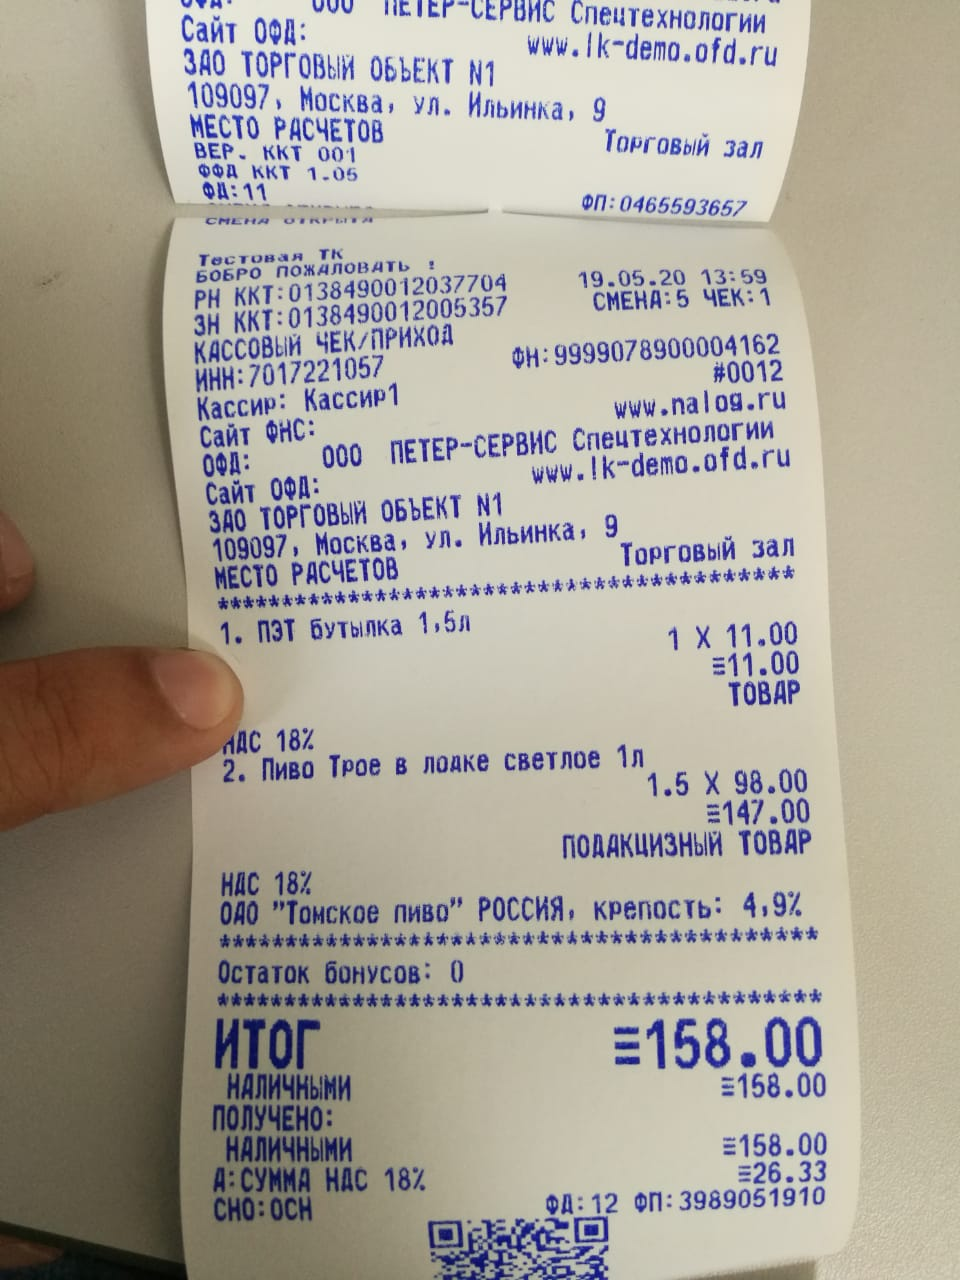
\includegraphics[width=225pt]{1.jpeg}} at (0pt,0pt)
\end{tikzpicture}
    ;\par
    3. Табличная часть <<Товары>> в форме рабочего места кассира очистится;\par
    4. Поле <<СНО>> в чеке имеет значение <<ОСН>>&  \\
    \hline
    %****************************************************************************************************


\end{longtable}
